\documentclass{beamer}
\usetheme{metropolis}           % Use metropolis theme

% ---------------------
%    PREAMBLE
% ---------------------
\usepackage[utf8]{inputenc}
\usepackage{inconsolata}

\usepackage{booktabs} % For professional looking tables
\usepackage{multirow}
\usepackage{adjustbox}

\usepackage{float}
\usepackage{tikz}
\usepackage{pgfplots}
\usepgfplotslibrary{dateplot}
\pgfplotsset{compat=1.9}

% Copyright 2017 Sergei Tikhomirov, MIT License
% https://github.com/s-tikhomirov/solidity-latex-highlighting/

\usepackage[final]{listings}
\usepackage{xcolor}

\definecolor{verylightgray}{rgb}{.97,.97,.97}

\lstdefinelanguage{Solidity}{
	keywords=[1]{anonymous, assembly, assert, balance, break, call, callcode, case, catch, class, constant, continue, contract, debugger, default, delegatecall, delete, do, else, emit, event, export, external, false, finally, for, function, gas, if, implements, import, in, indexed, instanceof, interface, internal, is, length, library, log0, log1, log2, log3, log4, memory, modifier, new, payable, pragma, private, protected, public, pure, push, require, return, returns, revert, selfdestruct, send, storage, struct, suicide, super, switch, then, this, throw, transfer, true, try, typeof, using, value, view, while, with, addmod, ecrecover, keccak256, mulmod, ripemd160, sha256, sha3}, % generic keywords including crypto operations
	keywordstyle=[1]\color{blue}\bfseries,
	keywords=[2]{address, bool, byte, bytes, bytes1, bytes2, bytes3, bytes4, bytes5, bytes6, bytes7, bytes8, bytes9, bytes10, bytes11, bytes12, bytes13, bytes14, bytes15, bytes16, bytes17, bytes18, bytes19, bytes20, bytes21, bytes22, bytes23, bytes24, bytes25, bytes26, bytes27, bytes28, bytes29, bytes30, bytes31, bytes32, enum, int, int8, int16, int24, int32, int40, int48, int56, int64, int72, int80, int88, int96, int104, int112, int120, int128, int136, int144, int152, int160, int168, int176, int184, int192, int200, int208, int216, int224, int232, int240, int248, int256, mapping, string, uint, uint8, uint16, uint24, uint32, uint40, uint48, uint56, uint64, uint72, uint80, uint88, uint96, uint104, uint112, uint120, uint128, uint136, uint144, uint152, uint160, uint168, uint176, uint184, uint192, uint200, uint208, uint216, uint224, uint232, uint240, uint248, uint256, var, void, ether, finney, szabo, wei, days, hours, minutes, seconds, weeks, years},	% types; money and time units
	keywordstyle=[2]\color{teal}\bfseries,
	keywords=[3]{block, blockhash, coinbase, difficulty, gaslimit, number, timestamp, msg, data, gas, sender, sig, value, now, tx, gasprice, origin},	% environment variables
	keywordstyle=[3]\color{violet}\bfseries,
	identifierstyle=\color{black},
	sensitive=false,
	comment=[l]{//},
	morecomment=[s]{/*}{*/},
	commentstyle=\color{gray}\ttfamily,
	stringstyle=\color{red}\ttfamily,
	morestring=[b]',
	morestring=[b]"
}

\lstset{
	language=Solidity,
	backgroundcolor=\color{white},
	extendedchars=true,
	basicstyle=\footnotesize\ttfamily,
	showstringspaces=false,
	showspaces=false,
	numbers=none,
	numberstyle=\footnotesize,
	numbersep=9pt,
	tabsize=2,
	breaklines=true,
	showtabs=false,
	captionpos=t
}

\usepackage[final]{listings}

\newcommand{\code}[1]{\texttt{#1}}
\newcommand{\dappaddress}[0]{\code{0xd82429497c69208a358ece305efc7aba4b237fe2}}
\newcommand{\gaspricegwei}[0]{$17.0111$ GWei }
\newcommand{\ethtoeur}[0]{$1 \text{ETH} = 537.2578 \text{EUR}$}
\newcommand{\dataseriesfull}{(2017-08-01, 1.93) (2017-08-02, 1.83) (2017-08-03, 1.86) (2017-08-04, 1.68) (2017-08-05, 2.03) (2017-08-06, 2.14) (2017-08-07, 2.26) (2017-08-08, 2.36) (2017-08-09, 2.40) (2017-08-10, 2.41) (2017-08-11, 2.56) (2017-08-12, 2.55) (2017-08-13, 2.19) (2017-08-14, 2.19) (2017-08-15, 2.11) (2017-08-16, 3.49) (2017-08-17, 2.92) (2017-08-18, 4.43) (2017-08-19, 2.57) (2017-08-20, 2.27) (2017-08-21, 2.48) (2017-08-22, 2.45) (2017-08-23, 2.46) (2017-08-24, 2.63) (2017-08-25, 2.75) (2017-08-26, 2.49) (2017-08-27, 2.51) (2017-08-28, 2.61) (2017-08-29, 3.15) (2017-08-30, 3.26) (2017-08-31, 4.59) (2017-09-01, 3.73) (2017-09-02, 7.22) (2017-09-03, 2.86) (2017-09-04, 2.76) (2017-09-05, 3.18) (2017-09-06, 4.02) (2017-09-07, 3.90) (2017-09-08, 4.22) (2017-09-09, 2.94) (2017-09-10, 3.47) (2017-09-11, 2.58) (2017-09-12, 2.72) (2017-09-13, 2.49) (2017-09-14, 2.01) (2017-09-15, 2.90) (2017-09-16, 2.85) (2017-09-17, 2.71) (2017-09-18, 2.61) (2017-09-19, 2.60) (2017-09-20, 2.79) (2017-09-21, 2.04) (2017-09-22, 2.12) (2017-09-23, 2.20) (2017-09-24, 2.62) (2017-09-25, 2.45) (2017-09-26, 2.33) (2017-09-27, 2.69) (2017-09-28, 2.50) (2017-09-29, 2.23) (2017-09-30, 2.60) (2017-10-01, 2.42) (2017-10-02, 2.52) (2017-10-03, 2.34) (2017-10-04, 2.33) (2017-10-05, 2.40) (2017-10-06, 2.66) (2017-10-07, 2.36) (2017-10-08, 2.48) (2017-10-09, 2.40) (2017-10-10, 2.51) (2017-10-11, 3.03) (2017-10-12, 2.47) (2017-10-13, 2.99) (2017-10-14, 2.71) (2017-10-15, 2.63) (2017-10-16, 1.85) (2017-10-17, 1.51) (2017-10-18, 1.48) (2017-10-19, 1.26) (2017-10-20, 1.48) (2017-10-21, 1.22) (2017-10-22, 1.07) (2017-10-23, 1.34) (2017-10-24, 1.44) (2017-10-25, 1.27) (2017-10-26, 1.24) (2017-10-27, 1.17) (2017-10-28, 1.06) (2017-10-29, 1.07) (2017-10-30, 1.22) (2017-10-31, 1.41) (2017-11-01, 1.48) (2017-11-02, 1.55) (2017-11-03, 1.33) (2017-11-04, 1.18) (2017-11-05, 1.08) (2017-11-06, 1.07) (2017-11-07, 1.34) (2017-11-08, 1.70) (2017-11-09, 1.72) (2017-11-10, 1.53) (2017-11-11, 1.65) (2017-11-12, 1.91) (2017-11-13, 1.77) (2017-11-14, 1.89) (2017-11-15, 1.95) (2017-11-16, 1.77) (2017-11-17, 1.83) (2017-11-18, 1.56) (2017-11-19, 1.69) (2017-11-20, 1.98) (2017-11-21, 2.13) (2017-11-22, 2.08) (2017-11-23, 2.19) (2017-11-24, 2.43) (2017-11-25, 1.99) (2017-11-26, 2.32) (2017-11-27, 2.49) (2017-11-28, 2.65) (2017-11-29, 2.49) (2017-11-30, 2.46) (2017-12-01, 2.27) (2017-12-02, 2.05) (2017-12-03, 2.16) (2017-12-04, 3.44) (2017-12-05, 4.81) (2017-12-06, 6.31) (2017-12-07, 9.03) (2017-12-11, 6.01) (2017-12-12, 8.53) (2017-12-13, 9.13) (2017-12-14, 9.86) (2017-12-15, 8.24) (2017-12-16, 8.31) (2017-12-17, 7.13) (2017-12-18, 7.33) (2017-12-19, 9.49) (2017-12-20, 11.22) (2017-12-21, 11.25) (2017-12-22, 9.10) (2017-12-23, 7.92) (2017-12-24, 6.90) (2017-12-25, 6.36) (2017-12-26, 6.67) (2017-12-27, 6.36) (2017-12-28, 5.87) (2017-12-29, 6.21) (2017-12-30, 5.85) (2017-12-31, 6.29) (2018-01-01, 5.94) (2018-01-02, 7.54) (2018-01-03, 8.83) (2018-01-04, 10.66) (2018-01-05, 27.82) (2018-01-06, 33.03) (2018-01-07, 27.79) (2018-01-08, 28.74) (2018-01-09, 34.54) (2018-01-10, 42.34) (2018-01-11, 31.98) (2018-01-12, 25.54) (2018-01-13, 29.82) (2018-01-14, 26.62) (2018-01-15, 23.02) (2018-01-16, 18.81) (2018-01-17, 17.23) (2018-01-18, 17.94) (2018-01-19, 17.28) (2018-01-20, 19.33) (2018-01-21, 13.68) (2018-01-22, 10.88) (2018-01-23, 12.47) (2018-01-24, 12.66) (2018-01-25, 11.32) (2018-01-26, 9.35) (2018-01-27, 9.57) (2018-01-28, 10.91) (2018-01-29, 13.79) (2018-01-30, 11.13) (2018-01-31, 9.89) (2018-02-01, 14.20) (2018-02-02, 11.39) (2018-02-03, 8.48) (2018-02-04, 8.65) (2018-02-05, 7.11) (2018-02-06, 6.10) (2018-02-07, 6.68) (2018-02-08, 6.04) (2018-02-09, 5.94) (2018-02-10, 6.68) (2018-02-11, 6.02) (2018-02-12, 5.48) (2018-02-13, 6.00) (2018-02-14, 5.99) (2018-02-15, 6.25) (2018-02-16, 6.32) (2018-02-17, 6.49) (2018-02-18, 7.08) (2018-02-19, 5.78) (2018-02-20, 5.97) (2018-02-21, 5.59) (2018-02-22, 4.63) (2018-02-23, 4.89) (2018-02-24, 5.37) (2018-02-25, 4.45) (2018-02-26, 4.80) (2018-02-27, 4.95) (2018-02-28, 5.65) (2018-03-01, 5.06) (2018-03-02, 5.62) (2018-03-03, 4.44) (2018-03-04, 4.68) (2018-03-05, 5.30) (2018-03-06, 4.88) (2018-03-07, 5.08) (2018-03-08, 4.39) (2018-03-09, 3.98) (2018-03-10, 3.37) (2018-03-11, 3.03) (2018-03-12, 3.51) (2018-03-13, 2.93) (2018-03-14, 3.09) (2018-03-15, 2.78) (2018-03-16, 3.21) (2018-03-17, 2.39) (2018-03-18, 2.29) (2018-03-19, 2.26) (2018-03-20, 2.38) (2018-03-21, 2.52) (2018-03-22, 2.58) (2018-03-23, 2.69) (2018-03-24, 2.37) (2018-03-25, 2.24) (2018-03-26, 3.01) (2018-03-27, 2.22) (2018-03-28, 2.09) (2018-03-29, 2.22) (2018-03-30, 1.58) (2018-03-31, 1.45) (2018-04-01, 1.41) (2018-04-02, 1.47) (2018-04-03, 1.52) (2018-04-04, 1.46) (2018-04-05, 1.89) (2018-04-06, 1.68) (2018-04-07, 1.28) (2018-04-08, 1.29) (2018-04-09, 1.52) (2018-04-10, 1.55) (2018-04-11, 1.63) (2018-04-12, 1.83) (2018-04-13, 2.44) (2018-04-14, 1.90) (2018-04-15, 1.82) (2018-04-16, 2.00) (2018-04-17, 1.97) (2018-04-18, 2.27) (2018-04-19, 2.11) (2018-04-20, 2.27) (2018-04-21, 2.14) (2018-04-22, 2.24) (2018-04-23, 2.43) (2018-04-24, 2.94) (2018-04-25, 3.08) (2018-04-26, 2.84) (2018-04-27, 3.14) (2018-04-28, 3.66) (2018-04-29, 3.37) (2018-04-30, 3.60) (2018-05-01, 3.09) (2018-05-02, 3.22) (2018-05-03, 3.65) (2018-05-04, 3.78) (2018-05-05, 3.44) (2018-05-06, 3.63) (2018-05-07, 3.53) (2018-05-08, 4.01) (2018-05-09, 3.72) (2018-05-10, 4.56) (2018-05-11, 4.45) (2018-05-12, 3.00) (2018-05-13, 3.24) (2018-05-14, 4.41) (2018-05-15, 4.42) (2018-05-16, 4.29) (2018-05-17, 4.45) (2018-05-18, 4.17) (2018-05-19, 4.08) (2018-05-20, 3.87) (2018-05-21, 4.23) (2018-05-22, 4.47) (2018-05-23, 4.24) (2018-05-24, 3.62) (2018-05-25, 3.68) (2018-05-26, 3.11) (2018-05-27, 2.90) (2018-05-28, 4.07) (2018-05-29, 3.68) (2018-05-30, 4.11) (2018-05-31, 4.88) (2018-06-01, 4.29) (2018-06-02, 3.12) (2018-06-03, 3.04) (2018-06-04, 3.93) (2018-06-05, 3.40) (2018-06-06, 3.99) (2018-06-07, 3.40) (2018-06-08, 3.17) (2018-06-09, 2.49) (2018-06-10, 2.44) (2018-06-11, 2.44) (2018-06-12, 2.49) (2018-06-13, 2.40) (2018-06-14, 2.52) (2018-06-15, 2.96) (2018-06-16, 4.09) (2018-06-17, 1.88) (2018-06-18, 1.98) (2018-06-19, 2.50)}

% ----------------
%    METADATA
% ----------------
\title{Docker as a service on the blockchain}
\date{July 20, 2018}
\author{Matteo Nardini}
\institute{Free University of Bolzano}

% ==================================

\begin{document}
    \maketitle

    \section{Introduction}
    \begin{frame}{Our goal}
        \centering
        Create a \emph{decentralized} market for computational power
    \end{frame}
    \begin{frame}{How}
        How:
        \begin{enumerate}
            \item Using Docker as a container engine to distribute computations
            \item Using the Ethereum blockchain as a basis for the decentralized market
        \end{enumerate}
        \vspace{1pt}
        A blockchain is a tamper-proof distributed ledger. Smart contracts are applications whose state and code are stored on a blockchain, therefore inheriting all of its advantages.
    \end{frame}

    \section{Our solution}
    \begin{frame}{Our solution}
        \begin{itemize}
            \item Designing a protocol to exchange computation requests and rewards for executing them
            \item Adding to the protocol some mechanisms to avoid dishonest behaviours
            \item Creating a smart contract that implements this protocol
            \item Creating a client application able to interact with this smart contract
        \end{itemize}
    \end{frame}
    \begin{frame}{The protocol: standard scenario}
        \begin{figure}
            \begin{center}
                \includegraphics[width=\textwidth]{Figs/standard-part-1.png}
            \end{center}
        \end{figure}
    \end{frame}
    \begin{frame}{The protocol: standard scenario}
        \begin{figure}
            \begin{center}
                \includegraphics[width=\textwidth]{Figs/standard-part-2.png}
            \end{center}
        \end{figure}
    \end{frame}

    \begin{frame}{Problem}
        \centering
        How to ensure that something agreed on the blockchain is respected in real world?
    \end{frame}
    \begin{frame}{Solution}
        Solutions found in literature:
        \begin{enumerate}
            \item Periodic checkpoints
            \item Heartbeat protocol
            \item Garbled circuits
            \item Verifiable computing (PCPs, SNARKs)
        \end{enumerate}
        \centering
        TL;DR: None of them is adequate
    \end{frame}
    \begin{frame}{Solution}
        Our approach:
        \begin{enumerate}
            \item The protocol becomes adjudicated
            \item There is a trusted auditor
            \item There are economic incentives to encourage honest behaviour
        \end{enumerate}
    \end{frame}

    \begin{frame}{The protocol: standard scenario}
        \begin{figure}
            \begin{center}
                \includegraphics[width=\textwidth]{Figs/standard-part-2.png}
            \end{center}
        \end{figure}
    \end{frame}
    \begin{frame}{The protocol: auditor intervention}
        \begin{figure}
            \begin{center}
                \includegraphics[width=\textwidth]{Figs/result-rejected-part-1.png}
            \end{center}
        \end{figure}
    \end{frame}
    \begin{frame}{The protocol: auditor intervention}
        \begin{figure}
            \begin{center}
                \includegraphics[width=\textwidth]{Figs/result-rejected-part-2.png}
            \end{center}
        \end{figure}
    \end{frame}

    \section{Evaluation}
    \begin{frame}{Associated costs}
        Costs of executing standard scenario.
        \begin{table}[h!]
            \begin{adjustbox}{max width=\textwidth}
                \centering
                \begin{tabular}{c c c c}
                    \toprule
                    Party & Gas consumed [Units] & Ether cost [GWei] & Euro cost [€]\\ 
                    \midrule
                    Publisher & 167898 & 2856130.20 & 1.53 \\ Farmer & 226341 & 3850310.11 & 2.07 \\ Total & 394239 & 6706440.31 & 3.60 \\
                    \bottomrule
                \end{tabular}
            \end{adjustbox}
        \end{table}
        This table assumes a \code{gasPrice} of \gaspricegwei and an exchange rate between Ether and Euro of \ethtoeur.
    \end{frame}
    \begin{frame}{Costs are volatile}
        \begin{adjustbox}{max width=\textwidth}
            \centering
            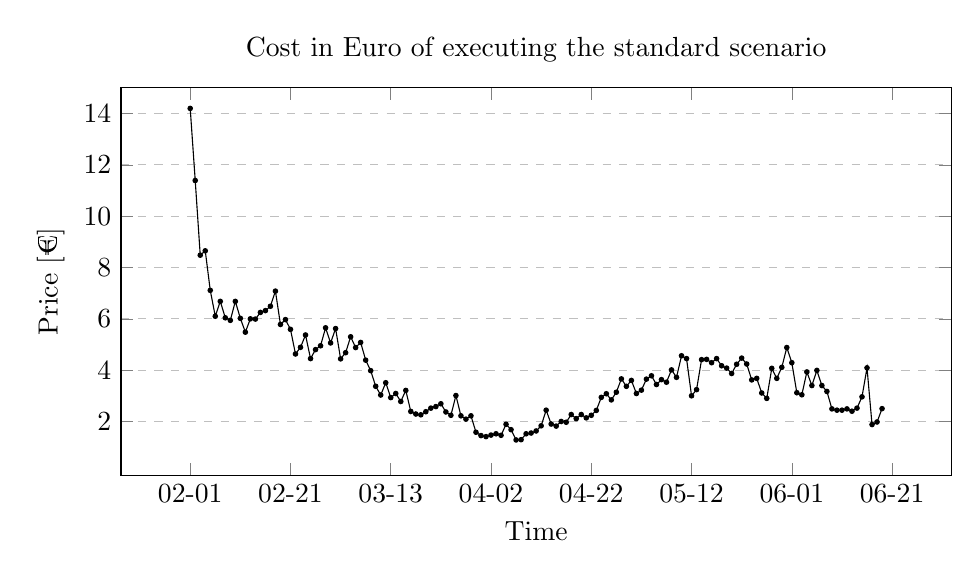
\begin{tikzpicture}
                \begin{axis} [
                    title={Cost in Euro of executing the standard scenario},
                    xlabel={Time}, ylabel={Price [€]},
                    ytick={2, 4, 6, 8, 10, 12, 14}, 
                    ymax=15,
                    ymajorgrids=true, grid style=dashed,
                    date coordinates in=x, date ZERO=2018-02-01,
                    xticklabel=\month-\day,
                    width=\textwidth, height=6.5cm
                ]

                \addplot[mark=*, mark size=0.8pt] coordinates {
                    (2018-02-01, 14.20) (2018-02-02, 11.39) (2018-02-03, 8.48) (2018-02-04, 8.65) (2018-02-05, 7.11) (2018-02-06, 6.10) (2018-02-07, 6.68) (2018-02-08, 6.04) (2018-02-09, 5.94) (2018-02-10, 6.68) (2018-02-11, 6.02) (2018-02-12, 5.48) (2018-02-13, 6.00) (2018-02-14, 5.99) (2018-02-15, 6.25) (2018-02-16, 6.32) (2018-02-17, 6.49) (2018-02-18, 7.08) (2018-02-19, 5.78) (2018-02-20, 5.97) (2018-02-21, 5.59) (2018-02-22, 4.63) (2018-02-23, 4.89) (2018-02-24, 5.37) (2018-02-25, 4.45) (2018-02-26, 4.80) (2018-02-27, 4.95) (2018-02-28, 5.65) (2018-03-01, 5.06) (2018-03-02, 5.62) (2018-03-03, 4.44) (2018-03-04, 4.68) (2018-03-05, 5.30) (2018-03-06, 4.88) (2018-03-07, 5.08) (2018-03-08, 4.39) (2018-03-09, 3.98) (2018-03-10, 3.37) (2018-03-11, 3.03) (2018-03-12, 3.51) (2018-03-13, 2.93) (2018-03-14, 3.09) (2018-03-15, 2.78) (2018-03-16, 3.21) (2018-03-17, 2.39) (2018-03-18, 2.29) (2018-03-19, 2.26) (2018-03-20, 2.38) (2018-03-21, 2.52) (2018-03-22, 2.58) (2018-03-23, 2.69) (2018-03-24, 2.37) (2018-03-25, 2.24) (2018-03-26, 3.01) (2018-03-27, 2.22) (2018-03-28, 2.09) (2018-03-29, 2.22) (2018-03-30, 1.58) (2018-03-31, 1.45) (2018-04-01, 1.41) (2018-04-02, 1.47) (2018-04-03, 1.52) (2018-04-04, 1.46) (2018-04-05, 1.89) (2018-04-06, 1.68) (2018-04-07, 1.28) (2018-04-08, 1.29) (2018-04-09, 1.52) (2018-04-10, 1.55) (2018-04-11, 1.63) (2018-04-12, 1.83) (2018-04-13, 2.44) (2018-04-14, 1.90) (2018-04-15, 1.82) (2018-04-16, 2.00) (2018-04-17, 1.97) (2018-04-18, 2.27) (2018-04-19, 2.11) (2018-04-20, 2.27) (2018-04-21, 2.14) (2018-04-22, 2.24) (2018-04-23, 2.43) (2018-04-24, 2.94) (2018-04-25, 3.08) (2018-04-26, 2.84) (2018-04-27, 3.14) (2018-04-28, 3.66) (2018-04-29, 3.37) (2018-04-30, 3.60) (2018-05-01, 3.09) (2018-05-02, 3.22) (2018-05-03, 3.65) (2018-05-04, 3.78) (2018-05-05, 3.44) (2018-05-06, 3.63) (2018-05-07, 3.53) (2018-05-08, 4.01) (2018-05-09, 3.72) (2018-05-10, 4.56) (2018-05-11, 4.45) (2018-05-12, 3.00) (2018-05-13, 3.24) (2018-05-14, 4.41) (2018-05-15, 4.42) (2018-05-16, 4.29) (2018-05-17, 4.45) (2018-05-18, 4.17) (2018-05-19, 4.08) (2018-05-20, 3.87) (2018-05-21, 4.23) (2018-05-22, 4.47) (2018-05-23, 4.24) (2018-05-24, 3.62) (2018-05-25, 3.68) (2018-05-26, 3.11) (2018-05-27, 2.90) (2018-05-28, 4.07) (2018-05-29, 3.68) (2018-05-30, 4.11) (2018-05-31, 4.88) (2018-06-01, 4.29) (2018-06-02, 3.12) (2018-06-03, 3.04) (2018-06-04, 3.93) (2018-06-05, 3.40) (2018-06-06, 3.99) (2018-06-07, 3.40) (2018-06-08, 3.17) (2018-06-09, 2.49) (2018-06-10, 2.44) (2018-06-11, 2.44) (2018-06-12, 2.49) (2018-06-13, 2.40) (2018-06-14, 2.52) (2018-06-15, 2.96) (2018-06-16, 4.09) (2018-06-17, 1.88) (2018-06-18, 1.98) (2018-06-19, 2.50)
                };

                \end{axis}
            \end{tikzpicture}
        \end{adjustbox}
    \end{frame}
    \begin{frame}{Cat-astrophe}
        \begin{figure}
            \begin{adjustbox}{max width=\textwidth}
                \centering
                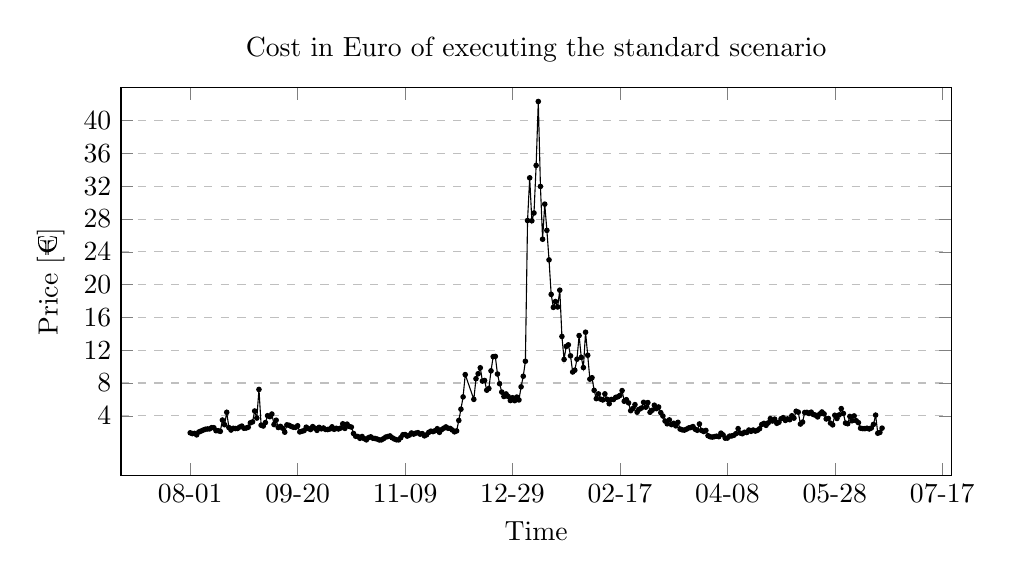
\begin{tikzpicture}
                    \begin{axis} [
                        title={Cost in Euro of executing the standard scenario},
                        xlabel={Time}, ylabel={Price [€]},
                        ytick={4, 8, 12, 16, 20, 24, 28, 32, 36, 40}, 
                        ymax=44,
                        ymajorgrids=true, grid style=dashed,
                        date coordinates in=x, date ZERO=2017-08-01,
                        xticklabel=\month-\day,
                        width=\textwidth, height=6.5cm
                    ]

                    \addplot[mark=*, mark size=0.8pt] coordinates {
                        \dataseriesfull    
                    };

                    \end{axis}
                \end{tikzpicture}
            \end{adjustbox}
        \end{figure}
    \end{frame}
    \begin{frame}{Cat-astrophe}
        \begin{figure}
            \begin{center}
                
\includegraphics[width=\textwidth]{Figs/cat-astrophe.jpg}
            \end{center}
        \end{figure}
    \end{frame}
    \begin{frame}{Conclusions}
        In conclusion:
        \begin{itemize}
            \item We developed a working prototype for this platform
            \item The protocol and the incentives should work
            \item The correct solution would have been verifiable computing
            \item Ethereum's blockchain costs are too high and too volatile
        \end{itemize}
        \centering
        TL;DR: Does this work? Not yet.
    \end{frame}
    \begin{frame}{Conclusions}
        \centering
        Thank you
    \end{frame}

    % EXTRA CONTENT
    \begin{frame}{Implementation details}
        \begin{figure}
            \begin{center}
                \includegraphics[width=\textwidth]{Figs/computation-states.png}
            \end{center}
        \end{figure}
    \end{frame}
    \begin{frame}[fragile]{Implementation details}
        \begin{center}
            \begin{lstlisting}
function acceptComputation(uint id) public {
    Computation storage c = computations[id];
    require(c.publisher != address(0), "Computation does not exists");
    require(c.status == Status.CREATED, "Status not correct");

    c.assignedTo = msg.sender;
    c.assignationTimestamp = block.timestamp;
    c.status = Status.ASSIGNED;

    emit ComputationAssigned(msg.sender, id);
}
            \end{lstlisting}
        \end{center}
    \end{frame}

\end{document}
